\documentclass[paper=a4,fontsize=11pt]{article}
\usepackage{amsmath,amssymb,amsthm}
\usepackage[protrusion=true,expansion=true]{microtype}	
\usepackage{algorithm}
\usepackage{algpseudocode}
\usepackage[margin=1.5in]{geometry}
\usepackage{graphicx}
\setlength{\textfloatsep}{0.1cm}
\setlength{\floatsep}{0.1cm}
\begin{document}
\title{TCSS 343 - Assignment 3}
\author{Jake McKenzie}
\maketitle
\section{UNDERSTAND}
In this problem use the Master Theorem to find and prove tight bounds for these recurrences (6 points each).\\\\
To solve this problem I used the master theorem taken from CLRS. I used a bit of a stronger statement than what was stated in the theorem but they are equivalent mathematically due to the nature of limits. I will include the theorem for the reader's benefit. To check my work I decided to include what I obtained using the Akra-Bazzi method.\\
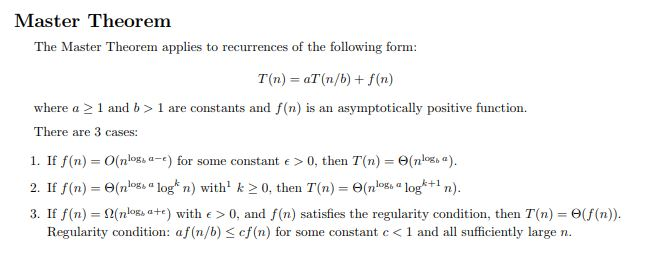
\includegraphics[width=\linewidth]{mastertheorem.JPG}
\begin{enumerate}
\item
\[
T(n) = \left\{
\begin{array}{cl}
c & \textrm{ if } n < 8\\
16T(\frac{n}{8}) + n\log{n} & \textrm{ if } n \geq 8
\end{array}
\right.
\]
By Master Method I obtain case 1:
\begin{align*}
\lim_{n\to\infty}{\frac{n\log{n}}{n^{\log_{8}{16}+\varepsilon}}}&=\lim_{n\to\infty}{\frac{n\log{n}}{n^{\frac{4}{3}+\frac{2}{3}}}}\\
&=\lim_{n\to\infty}{(\frac{n}{n})(\frac{\log{n}}{n})}\rightarrow0\\
T(n)&\in\Theta(n^{\frac{4}{3}})
\end{align*}
By Akra-Bazzi I obtain:\\
\begin{align*}
16(\frac{1}{8})^{p}&=1\\
p&=\frac{4}{3}
\end{align*}
\begin{align*}
T(n) &\in \Theta(n^{p}(1+\int_{1}^{n}{\frac{u\log{u}}{u^{p+1}}du}))\\
&\in \Theta(-9n+10n^{\frac{4}{3}}-3n\log{n})\\
&\in \Theta(n^{\frac{4}{3}})\\
\end{align*}
\item
\[
T(n) = \left\{
\begin{array}{cl}
c & \textrm{ if } n < 4\\
8T(\frac{n}{4}) + n\log n & \textrm{ if } n \geq 4
\end{array}
\right.
\]
By Master Method I obtain case 2:
\begin{align*}
    \lim_{n\to\infty}{\frac{n^{\frac{1}{3}}}{n^{\log_{8}{2}+\varepsilon}}}&=\lim_{n\to\infty}{\frac{n^{\frac{1}{3}}}{n^{\frac{1}{3}}}}\\
    &=\lim_{n\to\infty}{1}\rightarrow1\\
    &\in \Theta(n^{\frac{1}{3}}\log{n})\\
\end{align*}
By Akra-Bazzi I obtain:
\begin{align*}
    2(\frac{1}{8})^{p}&=1\\
    p&=\frac{1}{3}
\end{align*}
\begin{align*}
    T(n) &\in \Theta(n^{p}(1+\int_{1}^{n}{\frac{u^{\frac{1}{3}}}{u^{p+1}}du}))\\
    &\in \Theta(n^{\frac{1}{3}}+n^{\frac{1}{3}}\log{n})\\
    &\in \Theta(n^{\frac{1}{3}}\log{n})\\
\end{align*}
\item
\[
T(n) = \left\{
\begin{array}{cl}
c & \textrm{ if } n < 2\\
3T(\frac{n}{2}) + 9^n & \textrm{ if } n \geq 2
\end{array}
\right.
\]
By Master Method I obtain case 3:
\begin{align*}
    \lim_{n\to\infty}{\frac{9^n}{n^{\log_{3}{2}+\varepsilon}}}&=\lim_{n\to\infty}{\frac{9^n}{n^{\frac{\log{2}}{\log{3}}-(\frac{\log{2}}{\log{3}} + 1)}}}\\
    &=\lim_{n\to\infty}{n9^n}\rightarrow\infty\\
    &\in \Theta(9^n)\\
\end{align*}
This recurrence is not well suited for Akra-Bazzi.
\item
\[
T(n) = \left\{
\begin{array}{cl}
c & \textrm{ if } n \leq 1\\
3T(\frac{3n}{5}) + n^2 & \textrm{ if } n > 1
\end{array}
\right.
\]
By Master Method I obtain case 1:
\begin{align*}
    \lim_{n\to\infty}{\frac{n^2}{n^{\log_{\frac{5}{3}}{3}+\varepsilon}}}&=\lim_{n\to\infty}{\frac{n^2}{n^{\log_{\frac{5}{3}}{3}+(3-\log_{\frac{5}{3}}{3})}}}\\
    &=\lim_{n\to\infty}{\frac{n^2}{n^3}}\rightarrow0\\
    \log_{\frac{5}{3}}{3}&=2.15066...\\
    &\in \Theta(n^{2.15066...})\\
\end{align*}
By Akra-Bazzi I obtain:
\begin{align*}
    3(\frac{3}{5})^{p}&=1\\
    p&=\log_{\frac{5}{3}}{3}
\end{align*}
\begin{align*}
    T(n) &\in \Theta(n^{p}(1+\int_{1}^{n}{\frac{u^{2}}{u^{p+1}}du}))\\
    &\in \Theta(7.63746 n^{2.15066...}-6.63746 n^{2})\\
    &\in \Theta(n^{2.15066...})\\
\end{align*}
\item
\[
T(n) = \left\{
\begin{array}{cl}
c & \textrm{ if } n \leq 1\\
3T(\frac{3n}{5}) + n^{2.5} & \textrm{ if } n > 1
\end{array}
\right.
\]
By Master Method I obtain case 3:
\begin{align*}
    \lim_{n\to\infty}{\frac{n^{2.5}}{n^{\log_{\frac{5}{3}}{3}+\varepsilon}}}&=\lim_{n\to\infty}{\frac{n^{2.5}}{n^{\log_{\frac{5}{3}}{3}+0.1}}}\\
    &=\lim_{n\to\infty}{\frac{n^2.5}{n^{2.25}}}\rightarrow\infty\\
    &=\lim_{n\to\infty}{n^{0.25...}}\rightarrow\infty\\
    &\in \Theta(n^{2.5})\\
\end{align*}
\end{enumerate}

\section{EXPLORE}
For the following problems stated as pseudo-code, let $A[\ell\dots r]$ denote the sublist of the integer list $A$ from the $\ell$-th to the $r$-th element inclusive, let Cubic($A[1\dots n]$) denote an algorithm that runs in time $\Theta(n^3)$, and let Swift($A[1\dots n]$) denote an algorithm that runs in time $\Theta(n\log(\log n))$.\\
{\ttfamily
$\phantom{A}$\\
$\phantom{---}$ Three($A[1\dots n]$)\\
$\phantom{--- ---}$ If $n \leq 1$ Then Return // nothing to do\\
$\phantom{--- ---}$ Cubic($A[1\dots n]$)\\
$\phantom{--- ---}$ Three($A[1\dots\lfloor\frac{n}{2}\rfloor]$)\\
$\phantom{--- ---}$ Three($A[\lfloor\frac{n}{4}\rfloor+1\dots \lfloor\frac{3n}{4}\rfloor]$)\\
$\phantom{--- ---}$ Three($A[\lfloor\frac{n}{2}\rfloor+1\dots n]$)\\
$\phantom{---}$ End Three.
}
\begin{enumerate}
\item [(6 points) 1.] State a recurrence that gives the complexity $T(n)$ for algorithm \texttt{Three}.\\\\
For this problem I decided to analyze the cost of running each line individually.\\
{\ttfamily
$\phantom{A}$\\
$\phantom{---}$ Three($A[1\dots n]$) O(1)\\
$\phantom{--- ---}$ If $n \leq 1$ Then Return // nothing to do O(1)\\
$\phantom{--- ---}$ Cubic($A[1\dots n]$) O($n^3$)\\
$\phantom{--- ---}$ Three($A[1\dots\lfloor\frac{n}{2}\rfloor]$) T($\frac{n}{2}$)\\
$\phantom{--- ---}$ Three($A[\lfloor\frac{n}{4}\rfloor+1\dots \lfloor\frac{3n}{4}\rfloor]$) T($\frac{n}{2}$)\\
$\phantom{--- ---}$ Three($A[\lfloor\frac{n}{2}\rfloor+1\dots n]$) T($\frac{n}{2}$)\\
$\phantom{---}$ End Three. O(1)
}\\
Which gives me the following recurrece relation:\\
\[
T(n) = \left\{
\begin{array}{cl}
c & \textrm{ if } n \leq 1\\
3T(\frac{n}{2}) + n^3 & \textrm{ if } n > 1
\end{array}
\right.
\]
\item [(6 points) 2.] Find the tight complexity of algorithm \texttt{Three}.\\\\
By Master Theorem I obtain case 3:\\
\begin{align*}
    \lim_{n\to\infty}{\frac{n^3}{n^{\log{3}+\varepsilon}}}&=\lim_{n\to\infty}{\frac{n^3}{n^{\log{3}+(2 - \log{3})}}}\\
    &=\lim_{n\to\infty}{\frac{n^3}{n^2}}\\
    &=\lim_{n\to\infty}{n}\rightarrow\infty\\
    T(n)&\in \Theta(n^{3})\\
\end{align*}
By Akra-Bazzi I obtain:
\begin{align*}
    3(\frac{1}{2})^{p}&=1\\
    p&=\log_{2}{3}
\end{align*}
\begin{align*}
    T(n) &\in \Theta(n^{p}(1+\int_{1}^{n}{\frac{u^{3}}{u^{p+1}}du}))\\
    &\in \Theta(0.293305 n^{1.58496}+0.706695 n^{3})\\
    &\in \Theta(n^{3})\\
\end{align*}\\
{\ttfamily
$\phantom{A}$\\
$\phantom{---}$ One($A[1\dots n]$)\\
$\phantom{--- ---}$ If $n \leq 1$ Then Return // nothing to do\\
$\phantom{--- ---}$ Swift($A[1\dots n]$)\\
$\phantom{--- ---}$ One($A[1\dots\lfloor\frac{n}{2}\rfloor]$)\\
$\phantom{---}$ End One.
}\\
\item [(6 points) 3.] State a recurrence that gives the complexity $T(n)$ for algorithm \texttt{One}.\\
{\ttfamily
$\phantom{A}$\\
$\phantom{---}$ One($A[1\dots n]$)O(1)\\
$\phantom{--- ---}$ If $n \leq 1$ Then Return // nothing to do O(1)\\
$\phantom{--- ---}$ Swift($A[1\dots n]$)O($n\log{\log{n}}$)\\
$\phantom{--- ---}$ One($A[1\dots\lfloor\frac{n}{2}\rfloor]$) T($\frac{n}{2}$)\\
$\phantom{---}$ End One.
}\\
Which gives me the following recurrece relation:\\
\[
T(n) = \left\{
\begin{array}{cl}
c & \textrm{ if } n \leq 1\\
T(\frac{n}{2}) + n\log{\log{n}} & \textrm{ if } n > 1
\end{array}
\right.
\]
\item [(12 points) 4.] Find the tight complexity of algorithm \texttt{One}.\\
\begin{align*}
    \lim_{n\to\infty}{\frac{n\log{\log{n}}}{n^{\log{1}+\varepsilon}}}&=\lim_{n\to\infty}{\frac{n\log{\log{n}}}{n^{0+\gamma}}}\\
    \gamma&=0.577216\\
    &=\lim_{n\to\infty}{n^{0.422784}\log{\log{n}}}\rightarrow\infty\\
    T(n)&\in \Theta(n\log{\log{n}})\\
\end{align*}
By Akra-Bazzi I obtain:
\begin{align*}
    (\frac{1}{2})^{p}&=1\\
    p&=0
\end{align*}\\
As for computing this integral, it is non-elementary. It involes computing the $Li(u)$ which I've looked up and it defintely grows slower than any of the functions we normally use.\\\\
It's worth noting that we don't need to work about that, Akra-Bazzi tells us that if $p<k$ then we get case 3 of the master theorem.
\begin{align*}
    T(n) &\in \Theta(n^{p}(1+\int_{1}^{n}{\frac{u\log{\log{u}}}{u^{p+1}}du}))\\
    &\in \Theta(1 + \gamma - i \pi + n\log{\log{n}} - Li(n))\\
    &\in \Theta(n\log{\log{n}})\\
\end{align*}\\
\end{enumerate}
\section{PROGRAMMING}
Quicksort runs in it's worst case when it chooses the greatest or smallest element for each successive pivot. That recurrence relation can be written in the form of 

\[
T(n) = \left\{
\begin{array}{cl}
c & \textrm{ if } n < 1\\
T(n - 1) + O(n) & \textrm{ if } n \geq 1
\end{array}
\right.
\]
We've solved this recurrence relation plenty times before and the solution will just be stated as $\Theta(n^2)$. Now in practice was this what I obtained? By in large, on the 50 or so times I ran this program, this is what I obtained as a upper bound.\\\\
I was able to completely get rid of stackoverflows by implementing XORSwap, which is my favourite way to reduce the size of the stack. This is not the best swaping without a temporary variable routine in Java, arithmetic swap performs better due to compiler optimizations(arithmetic operators are used more often than bitwise ones so the compiler writers have written better optimizations for airthmetic) but it avoids overflows and leads to more desirable behaivor generally for this reason.\\\\
As for the space complexity I'm going to be honest and I couldn't make heads or tails of the space complexity of this algorithm from what I wrote. I think consulting the literature is important when this happens so here we go:\\\\
"For Quicksort, the combination of end- recursion removal and a policy of processing the smaller of the two subfiles first turns out to ensure that the stack need only contain room for about, lg N entries, since each entry on the stack after the top one must represent a subfile less than half the size of the previous entry." ~ Robert Sedgwick's Algorithms\\\\
There two possible correctors to this question of space complexity. $\log{n}$ and $n$ so which is it? Sedgwick seems to tell me it's $\log{n}$ which makes sense but if this true, why is that by implementing XORSwap I removed stackoverflows? Well let me consult James Aspnes lecture notes from a Computational Complexity Theory at Yale:\\\\
"There is no overhead in space complexity (except possibly dealing with the issue of a non-writable input tape with multiple heads), but the time complexity of a computation can easily go from $T$ to $O(T^2)$.\\\\
(chapter 3 page 14 http://www.cs.yale.edu/homes/aspnes/classes/468/notes.pdf)
What this telling me is that space complexity is less fickle and due to the nature of how information is stored it really does matter what the constant is. By reducing the number of swaps by a 1/3 ten times in my program I considerably dropped the space quicksort was using on the stack. But in both cases it was $\Theta(\log{n})$ but inorder to run it I needed to worry about that constant.\\\\
The excution times and the code will be included below. It's worth noting here for the reader that I did implement XORShift to generate better random numbers. I think this is a best practice. Just from eyeballing it, before included it I was getting numbers that seemed a little too good. The runningtimes are more in line with what I expect with a more normally distributed set of numbers.\\\\
\newpage
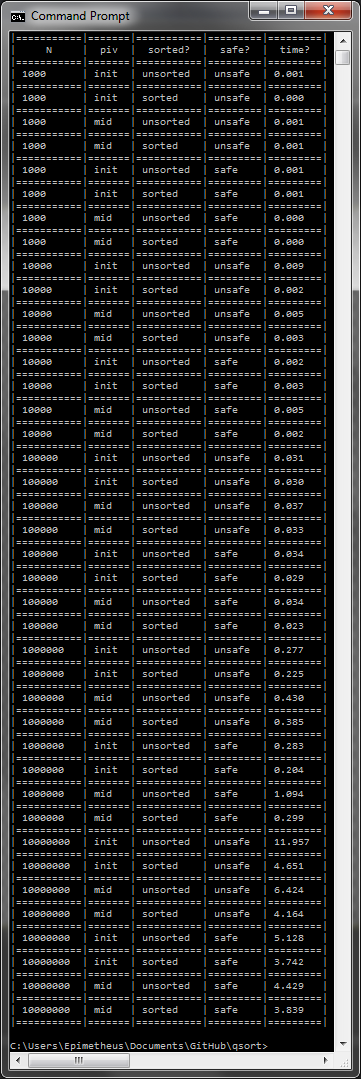
\includegraphics[scale = 2]{table.png}
\newpage
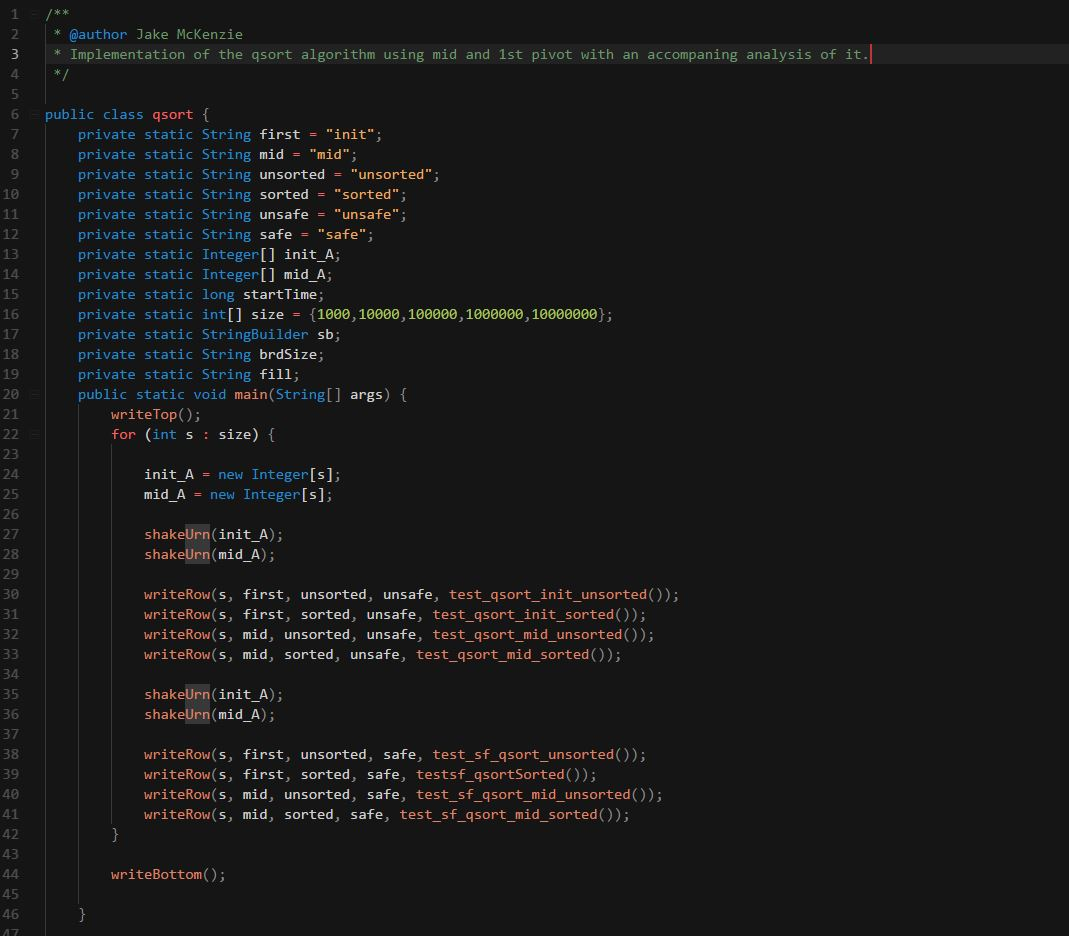
\includegraphics[width=\linewidth]{code1.jpg}
\newpage
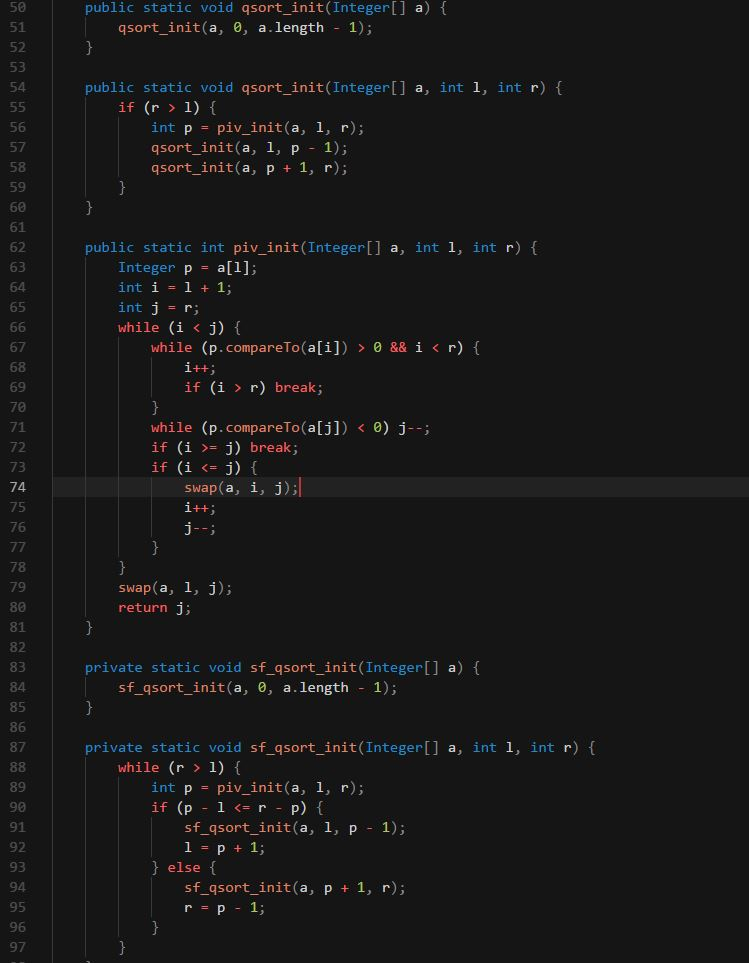
\includegraphics[width=\linewidth]{code2.jpg}
\newpage
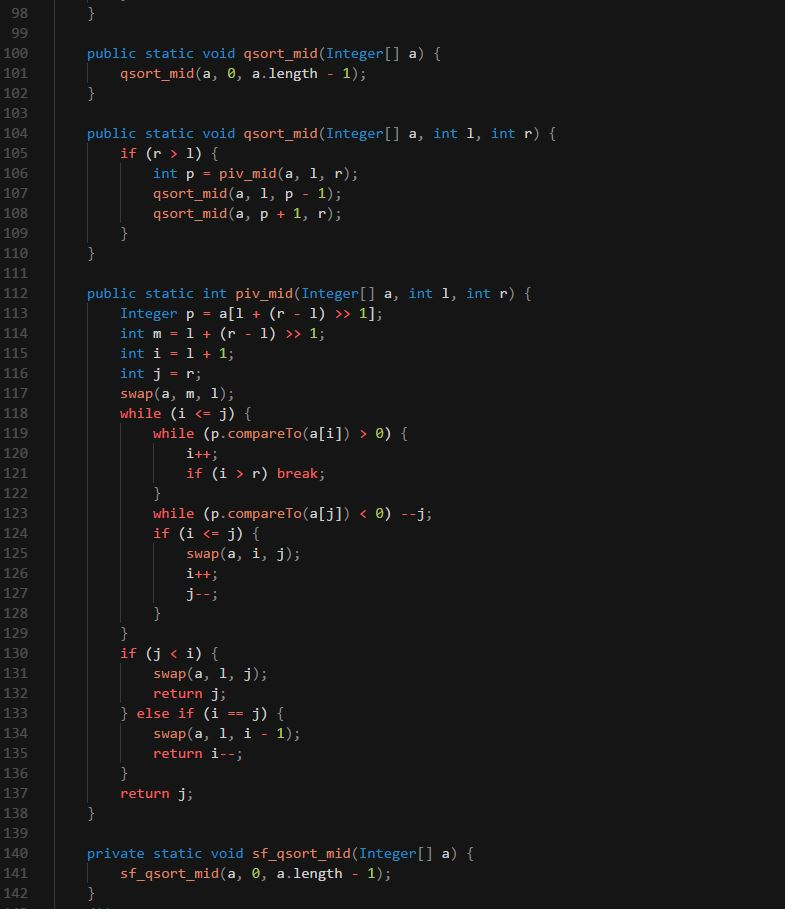
\includegraphics[width=\linewidth]{code3.jpg}
\newpage
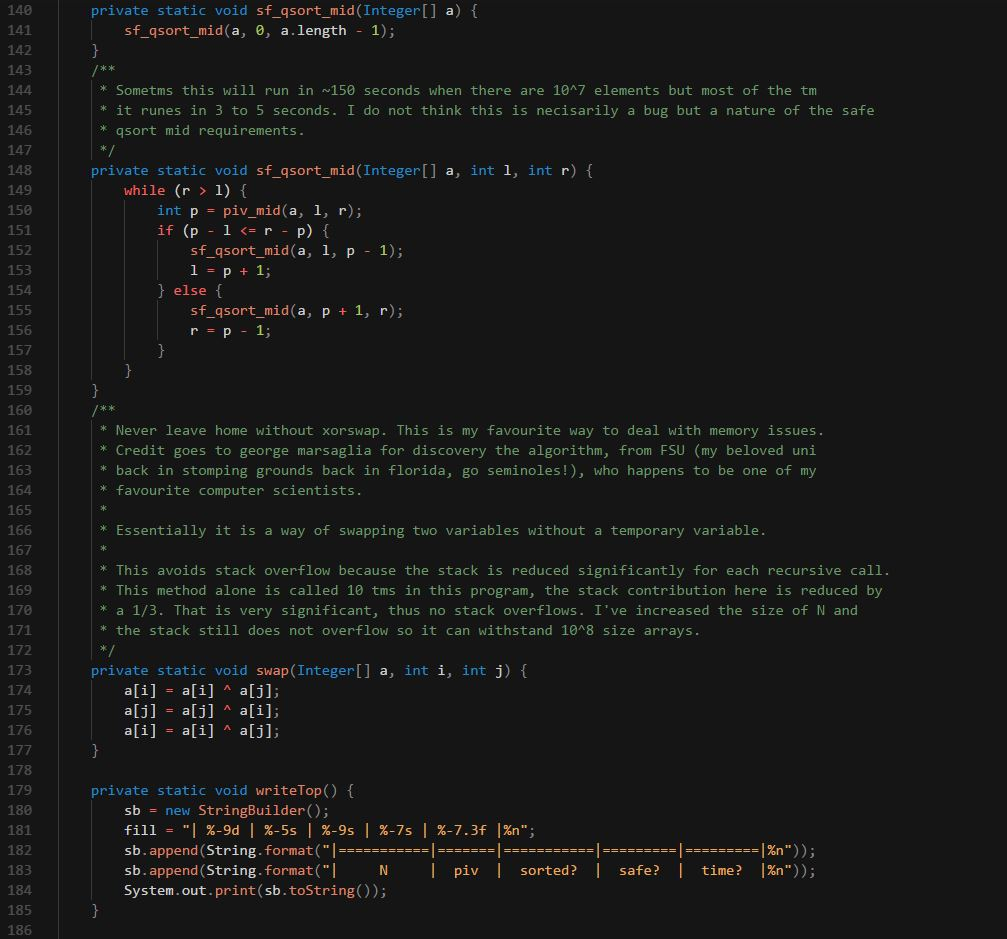
\includegraphics[width=\linewidth]{code4.jpg}
\newpage
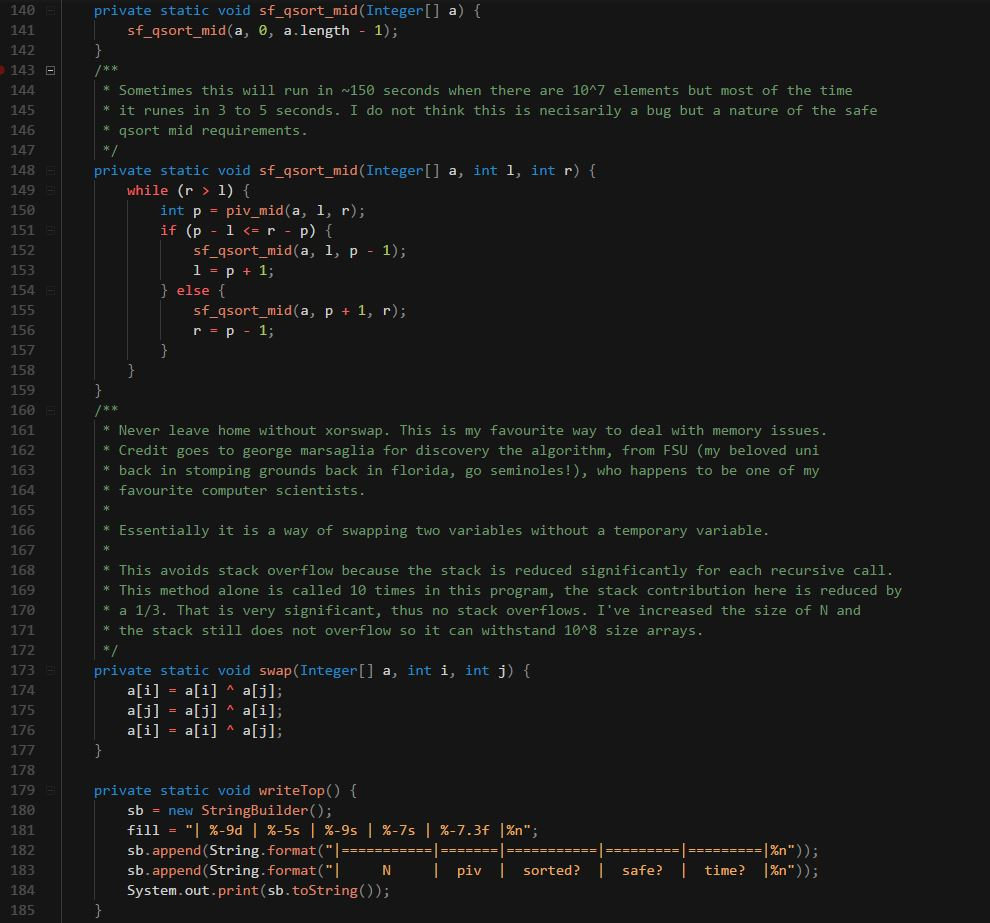
\includegraphics[width=\linewidth]{code5.jpg}
\newpage
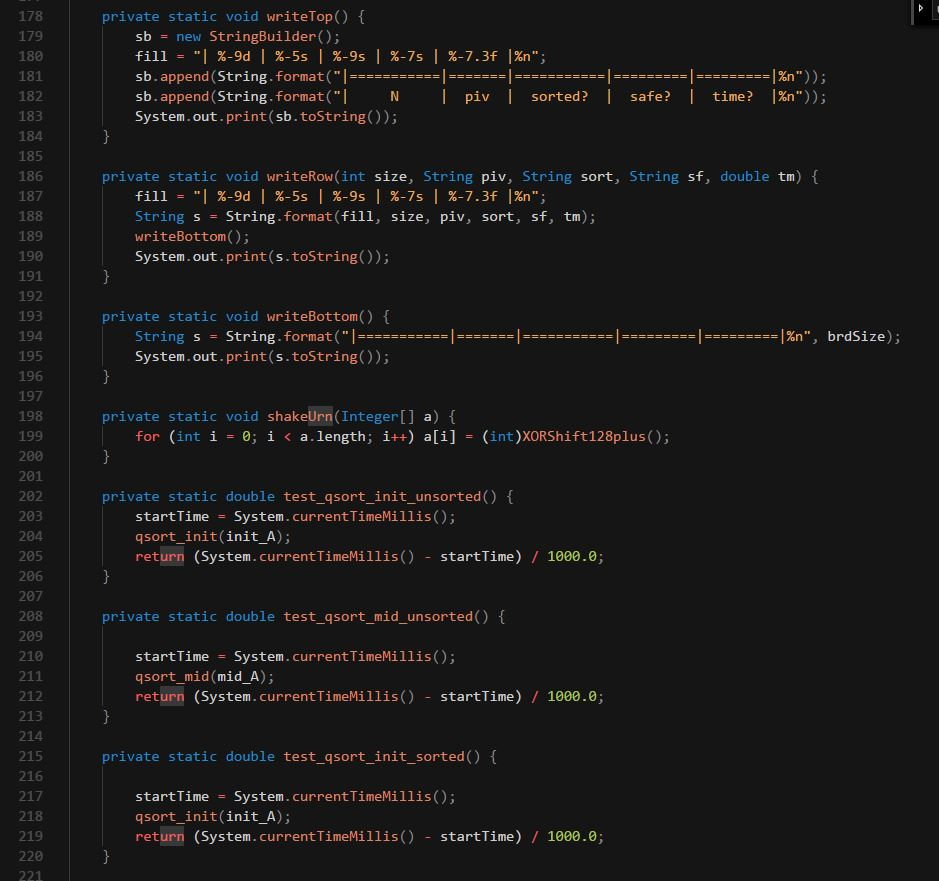
\includegraphics[width=\linewidth]{code6.jpg}
\newpage
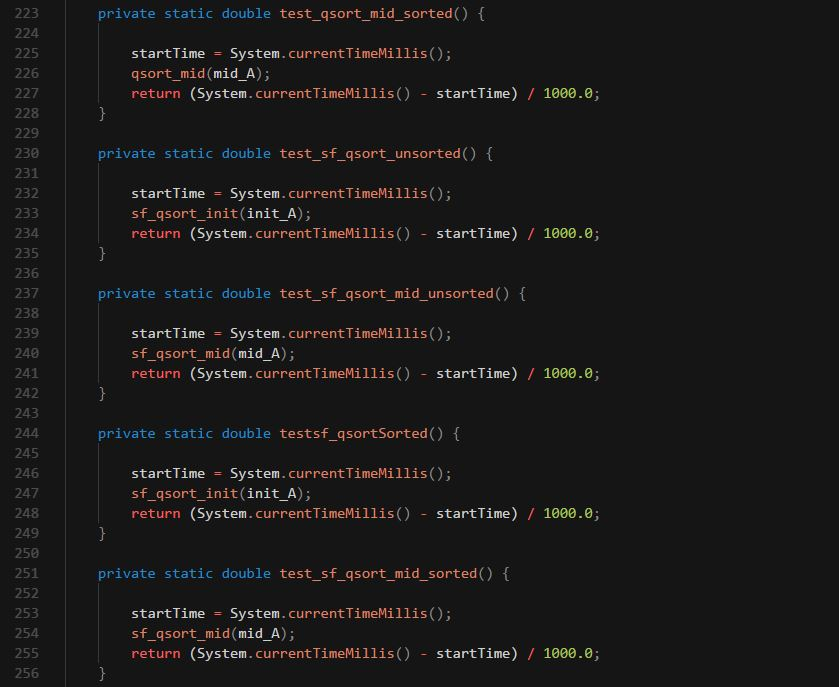
\includegraphics[width=\linewidth]{code7.jpg}
\newpage
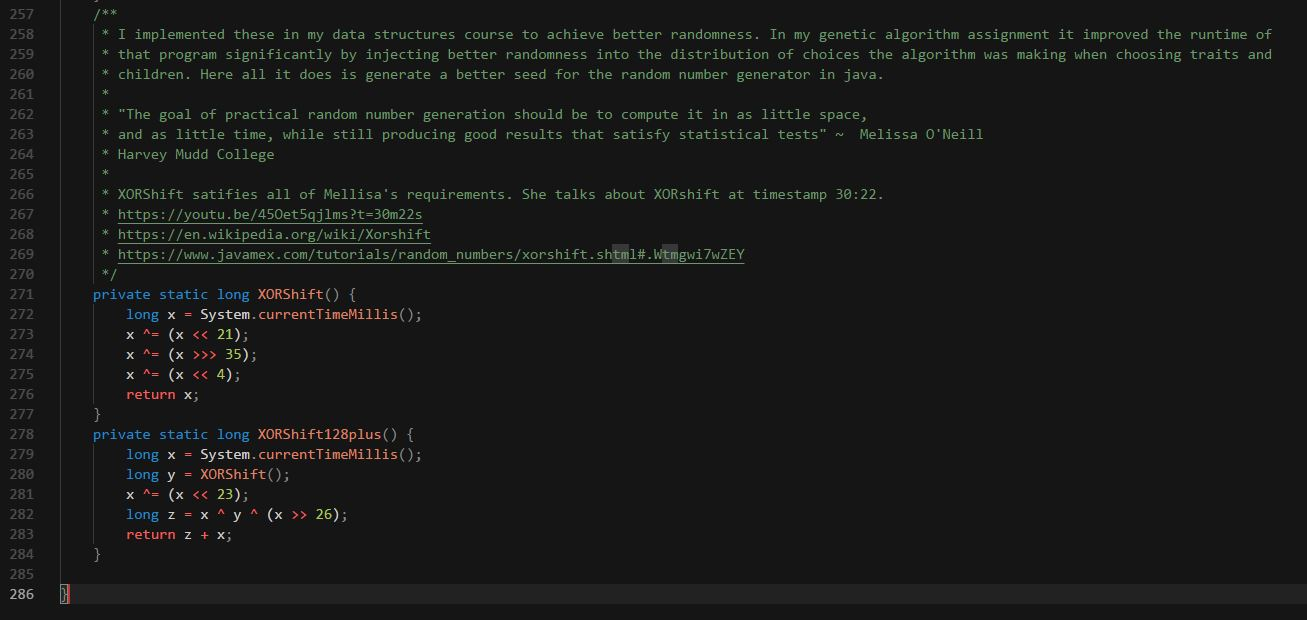
\includegraphics[width=\linewidth]{code8.jpg}
\newpage
\end{document}